\documentclass[conference]{IEEEtran}

\usepackage[utf8]{inputenc}
\usepackage{lmodern}
\usepackage[T1]{fontenc}
\usepackage[american]{babel}
\usepackage{amsmath}
\usepackage{amssymb}
\usepackage{microtype}

\usepackage{tikz,pgfplots}
\usetikzlibrary{arrows}
\usetikzlibrary{decorations.markings}
\pgfplotsset{compat=1.10} 
\usepackage{tikzscale}
\usepackage{booktabs}
\usepackage{nicefrac}
\usepackage{units}
%\usepackage[hyphens]{url}
\usepackage{tabu}
\usepackage{csquotes}
%\usepackage[load-configurations={abbreviations,binary}]{siunitx}
\usepackage[binary-units=true]{siunitx}
\usepackage[np]{numprint}
\usepackage{graphicx}
%\usepackage{subfig}
\usepackage{subfigure}
\npstyleenglish

%\usepackage[nowarn]{glossaries}
%\input{glossary.tex}

\usepackage[url=false,doi=false,backend=biber,style=ieee,sorting=none,maxnames=3]{biblatex}
\DeclareFieldFormat{labelnumberwidth}{\mkbibbold{#1.}}
\addbibresource{literature.bib}

\newcommand{\picwidth}{0.49\columnwidth}

\begin{document}
\title{YouTube Redundant Traffic}

%\numberofauthors{4}
%\author{
%\alignauthor Christian Moldovan\titlenote{This author is the one
%who did all the really hard work.}\\
%\affaddr{University of Duisburg-Essen}\\
%\affaddr{Modeling of Adaptive Systems}\\
%\affaddr{Essen, Germany}\\
%\email{christian.moldovan@uni-due.de}
%\alignauthor Christian Sieber\titlenote{This author is the one
%who did all the really hard work.}\\
%\affaddr{Technische Universität München}\\
%\affaddr{Chair of Communication Networks}\\
%\affaddr{Munich, Germany}\\
%\email{c.sieber@tum.de}
%\and
%\alignauthor Poul Heegaard\titlenote{This author is the one
%who did all the really hard work.}\\
%\affaddr{Norwegian University of Science and Technology}\\
%\affaddr{Department of Telematics}\\
%\affaddr{Trondheim, Norway}\\
%\email{poul.heegaard@item.ntnu.no}
%\alignauthor Tobias Hoßfeld\titlenote{This author is the one
%who did all the really hard work.}\\
%\affaddr{University of Duisburg-Essen}\\
%\affaddr{Modeling of Adaptive Systems}\\
%\affaddr{Essen, Germany}\\
%\email{tobias.hossfeld@uni-due.de}
%\alignauthor Wolfgang Kellerer\titlenote{This author is the one
%who did all the really hard work.}\\
%\affaddr{Technische Universität München}\\
%\affaddr{Chair of Communication Networks}\\
%\affaddr{Munich, Germany}\\
%\email{wolfgang.kellerer@tum.de}
%}

\author{
\IEEEauthorblockN{Christian Moldovan}\\
\IEEEauthorblockA{University of Duisburg-Essen\\
Modeling of Adaptive Systems\\
Essen, Germany\\
Email: christian.moldovan@uni-due.de}\\
\and
\IEEEauthorblockN{Christian Sieber}\\
\IEEEauthorblockA{Technische Universität München\\
Chair of Communication Networks\\
Munich, Germany\\
Email: c.sieber@tum.de}
\and
\IEEEauthorblockN{Poul Heegaard}\\
\IEEEauthorblockA{Norwegian University of Science and Technology\\
Department of Telematics\\
Trondheim, Norway
Email: poul.heegaard@item.ntnu.no}
\and
\IEEEauthorblockN{Tobias Hoßfeld}\\
\IEEEauthorblockA{University of Duisburg-Essen\\
Modeling of Adaptive Systems\\
Essen, Germany\\
Email: tobias.hossfeld@uni-due.de}
\and
\IEEEauthorblockN{Wolfgang Kellerer}\\
\IEEEauthorblockA{Technische Universität München\\
Chair of Communication Networks\\
Munich, Germany\\
Email: wolfgang.kellerer@tum.de}
}

%\author{Christian Moldovan \and Christian Sieber \and Poul Heegard \and Tobias Hoßfeld}
%\institute{University of Duisburg-Essen\\
%Modeling of Adaptive Systems\\
%Essen, Germany\\
%Email: 
%\email{christian.moldovan@uni-due.de},
%\email{c.sieber@tum.de},
%\email{poul.heegaard@item.ntnu.no},
%\email{tobias.hossfeld@uni-due.de}}

%\author{
%\IEEEauthorblockN{Christian Moldovan}
%\IEEEauthorblockA{University of Duisburg-Essen\\
%Modeling of Adaptive Systems\\
%Essen, Germany\\
%Email: christian.moldovan@uni-due.de}
%\and
%\IEEEauthorblockN{Florian Metzger}
%\IEEEauthorblockA{University of Duisburg-Essen\\
%Modeling of Adaptive Systems\\
%Essen, Germany\\
%Email: florian.metzger@uni-due.de}
%\and
%\IEEEauthorblockN{Tobias Hoßfeld}
%\IEEEauthorblockA{University of Duisburg-Essen\\
%Modeling of Adaptive Systems\\
%Essen, Germany\\
%Email: tobias.hossfeld@uni-due.de}
%}
% make the title area
\maketitle

%!TEX root = main.tex
%%%%%%%%%%%%%%%%%%%%%%%%%%%%%%%%%%%%%%%%%%%%%%%%%%%%%%%%%%%%%%%%%%%%%%%%%%%%%%%%

\begin{abstract}
\label{sec:abstract}
YouTube, as one of the major HTTP Adaptive Streaming video services, accounts for a large fraction of today's Internet traffic.
Therefore it is important to understand how efficiently YouTube uses the available network resources.
Previous work observed that the YouTube player replaces previously buffered segments with higher quality segments. This is good for the user as it increases the average quality level. 
However, the lower quality level segments are discarded and their traffic is redundant and therefore wasted.
In this paper, we use two independent approaches to evaluate the efficiency of YouTube's quality adaptation algorithm.
The first approach performs regression based on previously collected video views from a large experimental data set.
In the second approach we formulate a mixed integer linear program and calculate the optimal video quality adaptation. % considering the same bandwidth parameters and cumulative stalling times as the experimental data set.
The results show that the simplistic regression approach gives an accurate estimation of the optimal adaptation.
Furthermore, the optimization shows that the Quality of Experience (QoE)
% even when completely avoiding stalling, the quality level 
can be significantly improved compared to the actual average quality level observed in the real-world experiments, demanding for better video quality adaptation mechanisms by YouTube. 
%An outlook is provided on the potential that is left for improving YouTube's adaptation mechanism that is essential to managing the Quality of Experience of this important streaming service.
\end{abstract}



%!TEX root = main.tex
%%%%%%%%%%%%%%%%%%%%%%%%%%%%%%%%%%%%%%%%%%%%%%%%%%%%%%%%%%%%%%%%%%%%%%%%%%%%%%%%

\section{Introduction}
\label{sec:introduction}

mot1: growth of (adaptive) video streaming

mot2: with the growing competition in video streaming services, user expectations are also growing. Further, it is well known that stalling events and the video encoding bitrate (i.e. the video resolution) have a significant impact on the Acceptance Rate and the QoE \cite{casas2012youtube}.

what:

how

main contribution: we show there there is a lot of room for optimization for the used adaptation algorithms. Even if we completely avoid stalling events, a higher mean video quality is achievable in most cases. The number of resolution switches can be reduced.

structure

%!TEX root = main.tex
%%%%%%%%%%%%%%%%%%%%%%%%%%%%%%%%%%%%%%%%%%%%%%%%%%%%%%%%%%%%%%%%%%%%%%%%%%%%%%%%

\section{Related Work}
\label{sec:relatedwork}

QoE Related Work:

\begin{itemize}
\item \cite{casas2012youtube}
\item \cite{sieber16sacrificing,sieber15costaggressive}
\end{itemize}

YouTube Related Work:

\begin{itemize}
\item \cite{Anorga2015}
\item \cite{Yao2014b}
\item \cite{liu2013comparative}
\item \cite{Mansy2014}
\item \cite{nam2013mobile}
\item \cite{rao2011network}
\item \cite{ito14networklevel}
\item \cite{alcock11application}
\end{itemize}
%!TEX root = main.tex
%%%%%%%%%%%%%%%%%%%%%%%%%%%%%%%%%%%%%%%%%%%%%%%%%%%%%%%%%%%%%%%%%%%%%%%%%%%%%%%%

\section{System Model}
\label{sec:sysmodel}

\begin{figure}
\centering
\subfigure[$v_1$ = \_pjBVUyq530]{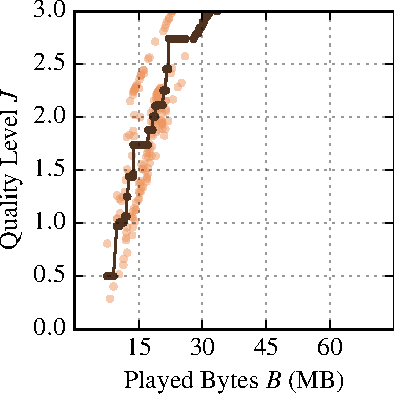
\includegraphics[width=0.45\columnwidth]{figs/32__pjBVUyq530.pdf}\label{fig:g1}}
\subfigure[$v_2$ = vbLLqaa9ksw]{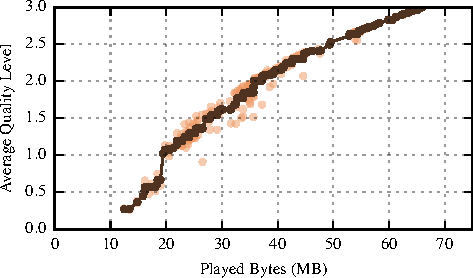
\includegraphics[width=0.45\columnwidth]{figs/32_vbLLqaa9ksw.pdf}\label{fig:g2}}
\caption{Approximated function $\theta$ for two of the videos.}
\vspace{-0.9em} 
\label{fig:regression}
\end{figure}
%!TEX root = main.tex
%%%%%%%%%%%%%%%%%%%%%%%%%%%%%%%%%%%%%%%%%%%%%%%%%%%%%%%%%%%%%%%%%%%%%%%%%%%%%%%%

\section{Results}
\label{sec:results}

\begin{figure}[t]
\centering
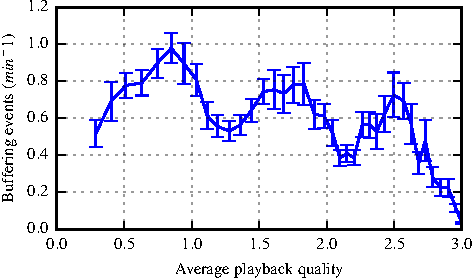
\includegraphics[width=0.95\linewidth]{figs/33qualityvstalling}%
\caption{Average playback quality versus stalling events}
\label{fig:qualityvsstalling}%
\end{figure}

Figure \ref{fig:qualityvsstalling} illustrates the relationship between the average quality level and the stalling events in the experiment result set.
For the average quality level, 0 is defined as \unit[100]{\%} of the segments are shown to the user in 144p. 3 is defined as \unit[100]{\%} of the segments are shown to the user in 480p.
The average quality levels are clustered using k-means and the error bars indicate the \unit[95]{\%} confidence interval of each cluster.
Two observations can be made from the figure. 
First, the lowest average quality level is 0.3 with about 0.5 switches per minute.
From this it follows that the player risks one stalling per two minutes in order to avoid showing only the lowest quality level in low bandwidth scenarios.
Second, the buffering events exhibit an oscillating behavior.
The oscillating behavior is consistent with observations made in \cite{sieber16sacrificing}.
The study shows that the behavior of YouTube's adaptation algorithm depends on the ratio between video bit-rate and available bandwidth.

In total, the pearson correlation shows a high correlation (-0.774) between average quality level and buffering events.

\subsection{optimal adaptation}

Idea: calculate the highest resolution that could have been achieved. compare it to measurement data. How much can still be gained?
opt was calculated according to the optimization problem in \cite{hossfeld2015identifying}. The calculations were done using the Gurobi Optimizer\footnote{http://www.gurobi.com/}.

In total we have four sets of results that we compare to each other:
\begin{itemize}
\item \textit{measurement}: the originally measured data set from \cite{sieber16sacrificing}; notice that stalling occured in these runs
\item \textit{opt (regression)}: assume that each segment is only downloaded once; same amount of stalling as measurement; was calculated in \cite{sieber16sacrificing}
\item \textit{opt (initial delay instead of stalling)}: gurobi (optimize mean quality based on \cite{hossfeld2015identifying}); same amount of stalling as measurement
\item \textit{opt (no stalling, no initial delay)}: gurobi (optimize mean quality based on \cite{hossfeld2015identifying}); no stalling
\end{itemize}


More details for \textit{opt (no stalling, no initial delay)}
\begin{itemize}
\item optimization done according to 2-step approach from \cite{miller2013optimal}
\item we assume no initial delay
\item this means, the total duration of a video session is lower if stalling occured in the measurement run. This means less total data is downloaded.
\end{itemize}
\textit{opt (initial delay instead of stalling)} was done similar to \textit{opt no stalling} with the difference that we added an initial delay $T_0$ to the replaying process. The duration of $T_0$ was equal to the total duration of all stalling events combined. This way, it is ensured that the same amount of data can be downloaded.

\begin{figure}[t]
\centering
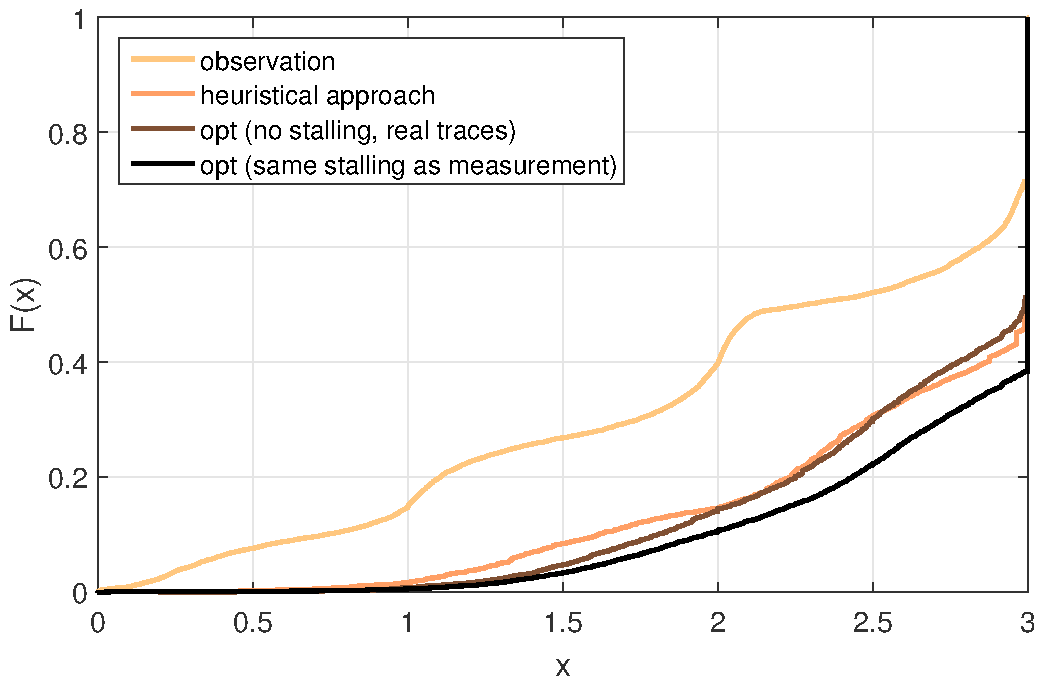
\includegraphics[width=0.5\textwidth]{figs/quality}%
\caption{CDF of the mean video quality in the measurement runs and highest achievable mean video quality according to the optimization problem in \cite{hossfeld2015identifying}. Remake figure!}
\label{fig:opt}%
\end{figure}

\begin{figure}[t]
\centering
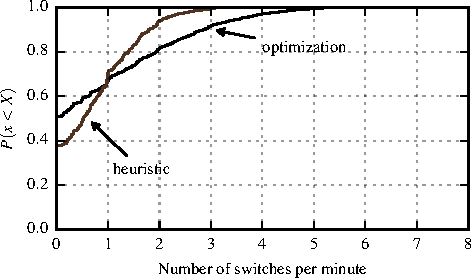
\includegraphics[width=0.5\textwidth]{figs/switches}%
\caption{CDF of the number of switches per minute. Remake figure!}
\label{fig:switches}%
\end{figure}

In figure \ref{fig:opt} we see the CDF of the mean video quality in the measurement runs and highest achievable mean video quality according to the optimization problem. In addition, we added an estimation of the avg. quality level that is possible based on downloaded data that was done in \cite{sieber16sacrificing}. While stalling events occured frequently during the original measurement, stalling events are not allowed to occur in the optimization problem. Therefore, we consider two sets of input for the opt. prob. for each measurement run: First, we only consider the available bandwidth during the video download. Second, we also respect the stalling events that occured. The sum of stalling was then added as initial delay during which the video was downloaded. In contrast to the YouTube measurement data where the video buffer does not contain more than 50s of video content at a time, in the calculations of the optimal adaptation we assumed that the video buffer is not limited.

%!TEX root = main.tex
%%%%%%%%%%%%%%%%%%%%%%%%%%%%%%%%%%%%%%%%%%%%%%%%%%%%%%%%%%%%%%%%%%%%%%%%%%%%%%%%

\section{Conclusion}
\label{sec:conclusion}

YouTube is a major source of Internet traffic world-wide and it is important to understand how it uses the available resources in a network.
Previous studies revealed that YouTube deploys a user-centric adaptation strategy which allows the player to discard previously downloaded segments and re-download them in a higher quality level.
This increases the average playback quality for the user, but in the same time decreases the overall efficiency.

In this paper we use two methods to quantify this decrease in efficiency.
The first methods is a fast heuristic approach based on historical data.
The second method is based on an optimization problem formulation.

Our results show there is still a lot of improvement possible for YouTube. Instead of downloading the same segment multiple times, the wasted traffic could be used to download segments in a higher quality. In average $20\%$ of the videos could have been downloaded in a higher quality. In spite of adaptive mechanisms, stalling usually occurred once per $1$ to $\SI{2}{\minute}$. Assuming the future network bandwidth can be predicted, our optimization problem shows that stalling can be prevented in $94\%$ of these cases. At the same time the initial delay can be kept below $\SI{10}{\second}$ in $95\%$ of cases. In future work, other streaming services such as Amazon Prime or Netflix may be investigated with the optimization approach described in this paper.


\printbibliography

%\input{notion}

\end{document}